\documentclass{standalone}
\usepackage{tikz}
\usetikzlibrary{patterns, positioning}

\begin{document}
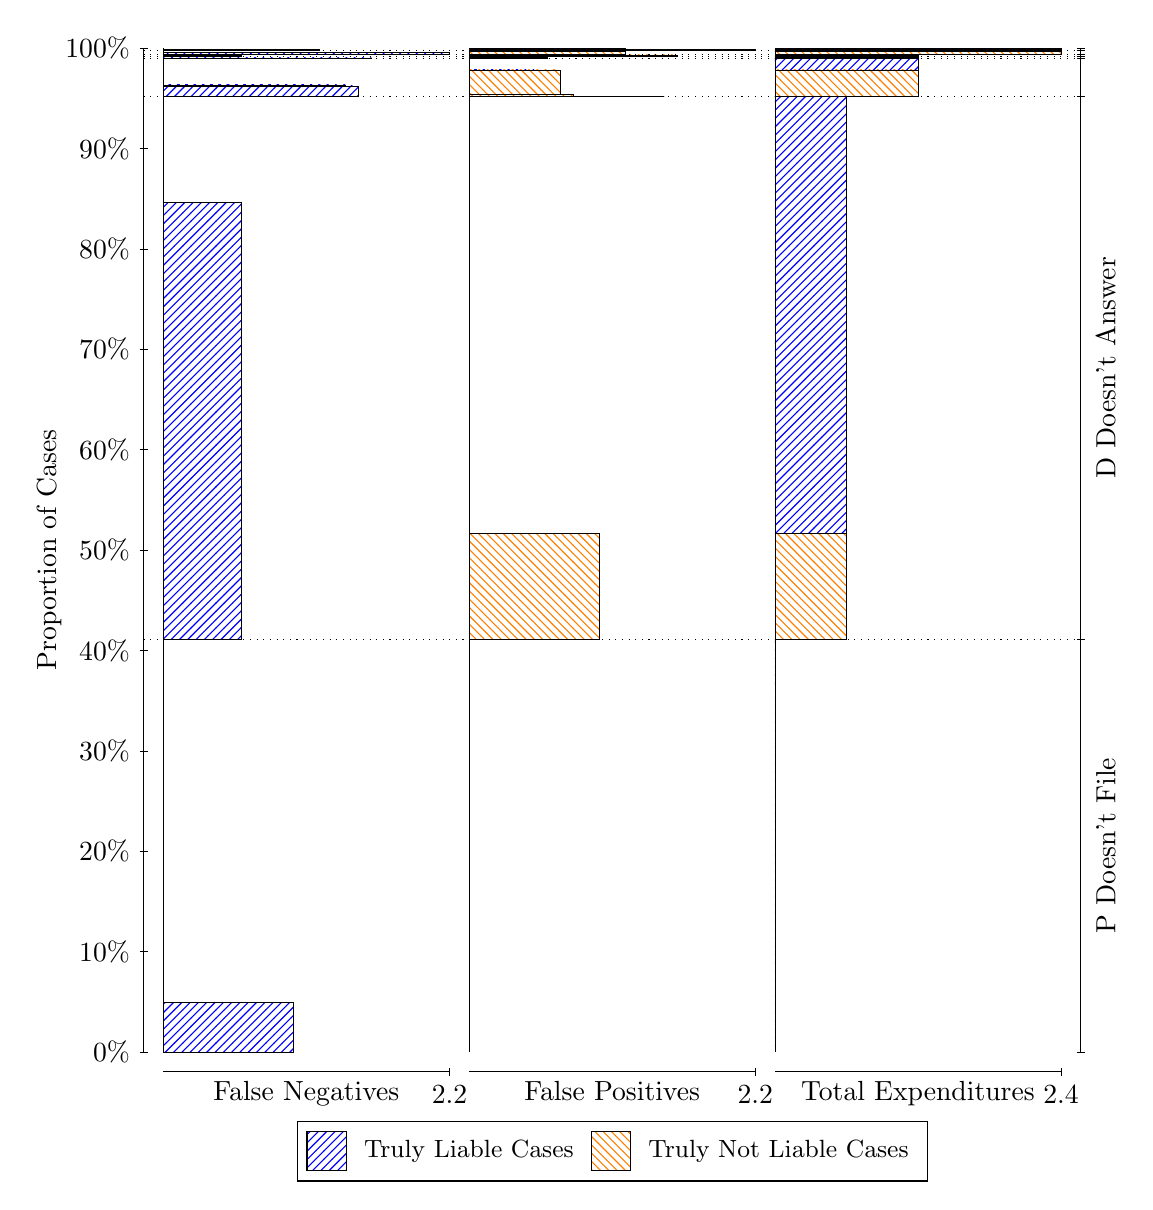
\begin{tikzpicture}
\draw[black, very thin] (1.5,1.75) -- (1.5,14.5);
\node[rotate=90, anchor=center] at (0.3, 8.125) {Proportion of Cases};
\draw[black, very thin] (1.45,1.75) -- (1.55,1.75);
\node[anchor=east] at (1.45, 1.75) {0\%};
\draw[black, very thin] (1.45,3.025) -- (1.55,3.025);
\node[anchor=east] at (1.45, 3.025) {10\%};
\draw[black, very thin] (1.45,4.3) -- (1.55,4.3);
\node[anchor=east] at (1.45, 4.3) {20\%};
\draw[black, very thin] (1.45,5.575) -- (1.55,5.575);
\node[anchor=east] at (1.45, 5.575) {30\%};
\draw[black, very thin] (1.45,6.85) -- (1.55,6.85);
\node[anchor=east] at (1.45, 6.85) {40\%};
\draw[black, very thin] (1.45,8.125) -- (1.55,8.125);
\node[anchor=east] at (1.45, 8.125) {50\%};
\draw[black, very thin] (1.45,9.4) -- (1.55,9.4);
\node[anchor=east] at (1.45, 9.4) {60\%};
\draw[black, very thin] (1.45,10.675) -- (1.55,10.675);
\node[anchor=east] at (1.45, 10.675) {70\%};
\draw[black, very thin] (1.45,11.95) -- (1.55,11.95);
\node[anchor=east] at (1.45, 11.95) {80\%};
\draw[black, very thin] (1.45,13.225) -- (1.55,13.225);
\node[anchor=east] at (1.45, 13.225) {90\%};
\draw[black, very thin] (1.45,14.5) -- (1.55,14.5);
\node[anchor=east] at (1.45, 14.5) {100\%};

\draw[black, very thin] (13.4,1.75) -- (13.4,14.5);
\draw[black, very thin] (13.35,1.75) -- (13.45,1.75);
\node[anchor=west] at (13.35, 1.75) {};
\draw[black, very thin] (13.35,6.989) -- (13.45,6.989);
\node[anchor=west] at (13.35, 6.989) {};
\draw[black, very thin] (13.35,13.885) -- (13.45,13.885);
\node[anchor=west] at (13.35, 13.885) {};
\draw[black, very thin] (13.35,14.368) -- (13.45,14.368);
\node[anchor=west] at (13.35, 14.368) {};
\draw[black, very thin] (13.35,14.395) -- (13.45,14.395);
\node[anchor=west] at (13.35, 14.395) {};
\draw[black, very thin] (13.35,14.423) -- (13.45,14.423);
\node[anchor=west] at (13.35, 14.423) {};
\draw[black, very thin] (13.35,14.473) -- (13.45,14.473);
\node[anchor=west] at (13.35, 14.473) {};
\draw[black, very thin] (13.35,14.5) -- (13.45,14.5);
\node[anchor=west] at (13.35, 14.5) {};

\draw[black, very thin, pattern color=blue, pattern=north east lines] (1.75,1.75) rectangle (3.4015,2.3788);
\draw[black, very thin, pattern color=orange, pattern=north west lines] (1.75,2.3788) rectangle (1.75,6.989);
\draw[black, very thin, pattern color=blue, pattern=north east lines] (1.75,6.989) rectangle (2.7409,12.539);
\draw[black, very thin, pattern color=orange, pattern=north west lines] (1.75,12.539) rectangle (1.75,13.885);
\draw[black, very thin, pattern color=blue, pattern=north east lines] (1.75,13.885) rectangle (4.2273,14.019);
\draw[black, very thin, pattern color=blue, pattern=north east lines] (1.75,14.019) rectangle (4.0621,14.031);
\draw[black, very thin, pattern color=blue, pattern=north east lines] (1.75,14.031) rectangle (3.897,14.032);
\draw[black, very thin, pattern color=blue, pattern=north east lines] (1.75,14.032) rectangle (3.7318,14.032);
\draw[black, very thin, pattern color=blue, pattern=north east lines] (1.75,14.032) rectangle (3.5667,14.032);
\draw[black, very thin, pattern color=blue, pattern=north east lines] (1.75,14.032) rectangle (3.4015,14.032);
\draw[black, very thin, pattern color=blue, pattern=north east lines] (1.75,14.032) rectangle (3.2364,14.032);
\draw[black, very thin, pattern color=blue, pattern=north east lines] (1.75,14.032) rectangle (3.0712,14.032);
\draw[black, very thin, pattern color=blue, pattern=north east lines] (1.75,14.032) rectangle (2.9061,14.032);
\draw[black, very thin, pattern color=orange, pattern=north west lines] (1.75,14.032) rectangle (1.75,14.368);
\draw[black, very thin, pattern color=blue, pattern=north east lines] (1.75,14.368) rectangle (4.3924,14.375);
\draw[black, very thin, pattern color=orange, pattern=north west lines] (1.75,14.375) rectangle (1.75,14.395);
\draw[black, very thin, pattern color=blue, pattern=north east lines] (1.75,14.395) rectangle (2.7409,14.407);
\draw[black, very thin, pattern color=orange, pattern=north west lines] (1.75,14.407) rectangle (1.75,14.423);
\draw[black, very thin, pattern color=blue, pattern=north east lines] (1.75,14.423) rectangle (5.3833,14.44);
\draw[black, very thin, pattern color=orange, pattern=north west lines] (1.75,14.44) rectangle (1.75,14.473);
\draw[black, very thin, pattern color=blue, pattern=north east lines] (1.75,14.473) rectangle (3.7318,14.487);
\draw[black, very thin, pattern color=orange, pattern=north west lines] (1.75,14.487) rectangle (1.75,14.5);
\draw[black, very thin, pattern color=orange, pattern=north west lines] (5.6333,1.75) rectangle (5.6333,6.3602);
\draw[black, very thin, pattern color=blue, pattern=north east lines] (5.6333,6.3602) rectangle (5.6333,6.989);
\draw[black, very thin, pattern color=orange, pattern=north west lines] (5.6333,6.989) rectangle (7.2848,8.3355);
\draw[black, very thin, pattern color=blue, pattern=north east lines] (5.6333,8.3355) rectangle (5.6333,13.885);
\draw[black, very thin, pattern color=orange, pattern=north west lines] (5.6333,13.885) rectangle (8.1106,13.885);
\draw[black, very thin, pattern color=orange, pattern=north west lines] (5.6333,13.885) rectangle (7.9455,13.885);
\draw[black, very thin, pattern color=orange, pattern=north west lines] (5.6333,13.885) rectangle (7.7803,13.885);
\draw[black, very thin, pattern color=orange, pattern=north west lines] (5.6333,13.885) rectangle (7.6152,13.885);
\draw[black, very thin, pattern color=orange, pattern=north west lines] (5.6333,13.885) rectangle (7.45,13.885);
\draw[black, very thin, pattern color=orange, pattern=north west lines] (5.6333,13.885) rectangle (7.2848,13.885);
\draw[black, very thin, pattern color=orange, pattern=north west lines] (5.6333,13.885) rectangle (7.1197,13.888);
\draw[black, very thin, pattern color=orange, pattern=north west lines] (5.6333,13.888) rectangle (6.9545,13.915);
\draw[black, very thin, pattern color=orange, pattern=north west lines] (5.6333,13.915) rectangle (6.7894,14.221);
\draw[black, very thin, pattern color=blue, pattern=north east lines] (5.6333,14.221) rectangle (6.4591,14.221);
\draw[black, very thin, pattern color=blue, pattern=north east lines] (5.6333,14.221) rectangle (6.2939,14.221);
\draw[black, very thin, pattern color=blue, pattern=north east lines] (5.6333,14.221) rectangle (6.1288,14.221);
\draw[black, very thin, pattern color=blue, pattern=north east lines] (5.6333,14.221) rectangle (5.9636,14.221);
\draw[black, very thin, pattern color=blue, pattern=north east lines] (5.6333,14.221) rectangle (5.7985,14.221);
\draw[black, very thin, pattern color=blue, pattern=north east lines] (5.6333,14.221) rectangle (5.6333,14.368);
\draw[black, very thin, pattern color=orange, pattern=north west lines] (5.6333,14.368) rectangle (6.6242,14.388);
\draw[black, very thin, pattern color=blue, pattern=north east lines] (5.6333,14.388) rectangle (5.6333,14.395);
\draw[black, very thin, pattern color=orange, pattern=north west lines] (5.6333,14.395) rectangle (8.2758,14.412);
\draw[black, very thin, pattern color=blue, pattern=north east lines] (5.6333,14.412) rectangle (6.6242,14.423);
\draw[black, very thin, pattern color=orange, pattern=north west lines] (5.6333,14.423) rectangle (7.6152,14.456);
\draw[black, very thin, pattern color=blue, pattern=north east lines] (5.6333,14.456) rectangle (5.9636,14.473);
\draw[black, very thin, pattern color=orange, pattern=north west lines] (5.6333,14.473) rectangle (9.2667,14.486);
\draw[black, very thin, pattern color=blue, pattern=north east lines] (5.6333,14.486) rectangle (7.6152,14.5);
\draw[black, very thin, pattern color=orange, pattern=north west lines] (9.5167,1.75) rectangle (9.5167,6.3602);
\draw[black, very thin, pattern color=blue, pattern=north east lines] (9.5167,6.3602) rectangle (9.5167,6.989);
\draw[black, very thin, pattern color=orange, pattern=north west lines] (9.5167,6.989) rectangle (10.425,8.3355);
\draw[black, very thin, pattern color=blue, pattern=north east lines] (9.5167,8.3355) rectangle (10.425,13.885);
\draw[black, very thin, pattern color=orange, pattern=north west lines] (9.5167,13.885) rectangle (11.333,13.885);
\draw[black, very thin, pattern color=blue, pattern=north east lines] (9.5167,13.885) rectangle (11.333,13.885);
\draw[black, very thin, pattern color=orange, pattern=north west lines] (9.5167,13.885) rectangle (11.333,14.221);
\draw[black, very thin, pattern color=blue, pattern=north east lines] (9.5167,14.221) rectangle (11.333,14.368);
\draw[black, very thin, pattern color=orange, pattern=north west lines] (9.5167,14.368) rectangle (11.333,14.368);
\draw[black, very thin, pattern color=blue, pattern=north east lines] (9.5167,14.368) rectangle (11.333,14.368);
\draw[black, very thin, pattern color=orange, pattern=north west lines] (9.5167,14.368) rectangle (11.333,14.388);
\draw[black, very thin, pattern color=blue, pattern=north east lines] (9.5167,14.388) rectangle (11.333,14.395);
\draw[black, very thin, pattern color=orange, pattern=north west lines] (9.5167,14.395) rectangle (11.333,14.412);
\draw[black, very thin, pattern color=blue, pattern=north east lines] (9.5167,14.412) rectangle (11.333,14.423);
\draw[black, very thin, pattern color=orange, pattern=north west lines] (9.5167,14.423) rectangle (13.15,14.456);
\draw[black, very thin, pattern color=blue, pattern=north east lines] (9.5167,14.456) rectangle (13.15,14.473);
\draw[black, very thin, pattern color=orange, pattern=north west lines] (9.5167,14.473) rectangle (13.15,14.486);
\draw[black, very thin, pattern color=blue, pattern=north east lines] (9.5167,14.486) rectangle (13.15,14.5);
\draw[black, dotted] (1.5,6.989) -- (13.4,6.989);
\draw[black, dotted] (1.5,13.885) -- (13.4,13.885);
\draw[black, dotted] (1.5,14.368) -- (13.4,14.368);
\draw[black, dotted] (1.5,14.395) -- (13.4,14.395);
\draw[black, dotted] (1.5,14.423) -- (13.4,14.423);
\draw[black, dotted] (1.5,14.473) -- (13.4,14.473);
\draw[black, very thin] (1.75,1.5) -- (5.3833,1.5);
\node[anchor=north] at (3.5667, 1.5) {False Negatives};
\draw[black, very thin] (5.3833,1.45) -- (5.3833,1.55);
\node[anchor=north] at (5.3833, 1.45) {2.2};

\draw[black, very thin] (5.6333,1.5) -- (9.2667,1.5);
\node[anchor=north] at (7.45, 1.5) {False Positives};
\draw[black, very thin] (9.2667,1.45) -- (9.2667,1.55);
\node[anchor=north] at (9.2667, 1.45) {2.2};

\draw[black, very thin] (9.5167,1.5) -- (13.15,1.5);
\node[anchor=north] at (11.333, 1.5) {Total Expenditures};
\draw[black, very thin] (13.15,1.45) -- (13.15,1.55);
\node[anchor=north] at (13.15, 1.45) {2.4};

\node[black, centered, rotate=90] at (13.72, 4.3695) {P Doesn't File};
\node[black, centered, rotate=90] at (13.72, 10.437) {D Doesn't Answer};






\draw (7.449999999999999,1.5) node[draw=none] (baseCoordinate) {};
\begin{scope}[align=center]
        \matrix[scale=0.5, draw=black, below=0.5cm of baseCoordinate, nodes={draw}, column sep=0.1cm]{
            \node[rectangle, draw, minimum width=0.5cm, minimum height=0.5cm, pattern=north east lines, pattern color=blue] {}; &
            \node[draw=none, font=\small] (B) {Truly Liable Cases}; &
            \node[rectangle, draw, minimum width=0.5cm, minimum height=0.5cm, pattern=north west lines, pattern color=orange] {}; &
            \node[draw=none, font=\small] (B) {Truly Not Liable Cases}; \\
            };
\end{scope}

\end{tikzpicture}
\end{document}